\section{Kết quả}
\label{sec:results}
\subsection{Độ chính xác trên ba tập}
\begin{table}[tbp]
\centering\scriptsize
\setlength{\tabcolsep}{3.5pt}
\begin{tabular}{lrrrrrrrrrrrr}
\toprule
& \multicolumn{4}{c}{Train} & \multicolumn{4}{c}{Validation} & \multicolumn{4}{c}{Test} \\
\cmidrule(lr){2-5}\cmidrule(lr){6-9}\cmidrule(lr){10-13}
Mô hình & Acc & P & R & F1 & Acc & P & R & F1 & Acc & P & R & F1 \\
\midrule
Gaussian NB & 80.13 & 81.85 & 79.74 & 79.98 & 79.67 & 81.39 & 79.27 & 79.50 & 81.32 & 82.98 & 80.95 & 81.16 \\
Softmax regression & 93.62 & 93.56 & 93.53 & 93.54 & 92.15 & 92.07 & 92.05 & 92.05 & 92.52 & 92.45 & 92.41 & 92.42 \\
MLP & 99.87 & 99.87 & 99.87 & 99.87 & 98.18 & 98.17 & 98.17 & 98.17 & 98.24 & 98.23 & 98.23 & 98.23 \\
AdaBoost-SAMME & 100.00 & 100.00 & 100.00 & 100.00 & 97.59 & 97.59 & 97.57 & 97.58 & 97.60 & 97.58 & 97.58 & 97.58 \\
CNN & 99.40 & 99.40 & 99.39 & 99.39 & 98.65 & 98.65 & 98.63 & 98.64 & 98.80 & 98.79 & 98.79 & 98.79 \\
\bottomrule
\end{tabular}

\caption{Accuracy, precision, recall và F1 macro (\%) trên train, validation và test (MNIST, seed 42).}
\label{tab:accuracy}
\end{table}

\Cref{tab:accuracy} cho thứ tự trên tập test: MLP (\accTestMLP\%) và AdaBoost (\accTestADA\%) vượt xa softmax (\accTestSM\%) và Naïve Bayes (\accTestNB\%). F1 macro lệch accuracy không quá $0.16$ điểm vì các lớp gần cân bằng. AdaBoost đạt $100\%$ trên train còn MLP đạt $99.87\%$, nên hai mô hình này khớp rất sát dữ liệu huấn luyện (chênh train--test $2.40$ và $1.63$ điểm). Softmax chỉ đạt $93.62\%$ trên train, tức bị giới hạn bởi biên tuyến tính. Naïve Bayes có test cao hơn train ($-1.19$ điểm). Mỗi mô hình chỉ được huấn luyện một lần nên khoảng cách giữa MLP và AdaBoost ($0.64$ điểm) chưa đủ để kết luận mô hình nào tốt hơn.

\begin{figure}[tbp]
\centering
\begin{subfigure}{0.325\textwidth}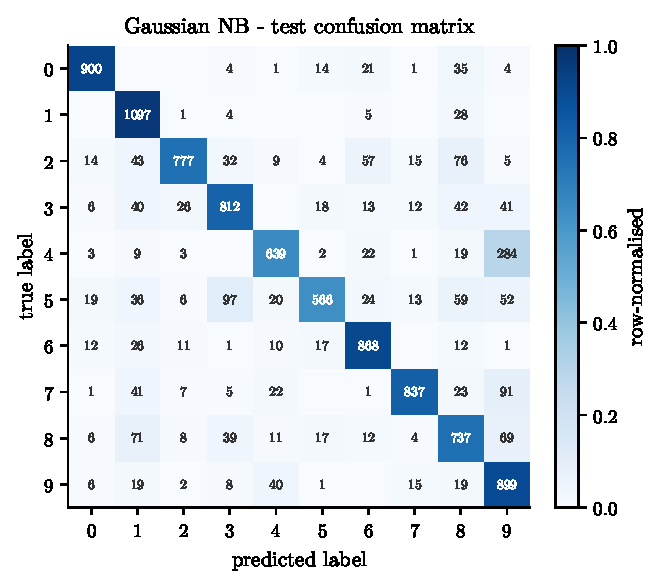
\includegraphics[width=\linewidth]{../results/figures/confusion_naive_bayes.pdf}\caption{Naïve Bayes}\end{subfigure}\hfill
\begin{subfigure}{0.325\textwidth}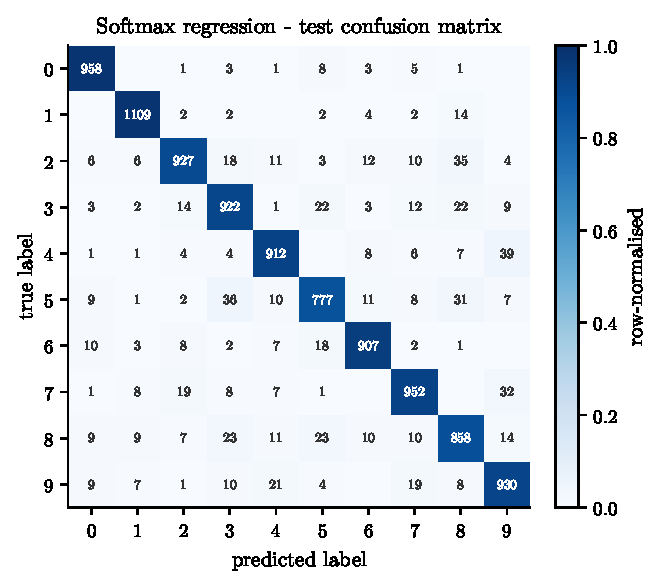
\includegraphics[width=\linewidth]{../results/figures/confusion_softmax.pdf}\caption{Softmax}\end{subfigure}\hfill
\begin{subfigure}{0.325\textwidth}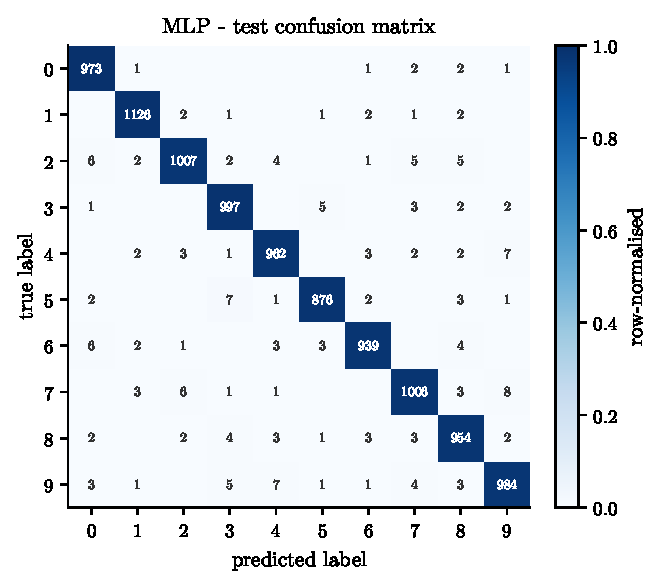
\includegraphics[width=\linewidth]{../results/figures/confusion_mlp.pdf}\caption{MLP}\end{subfigure}\\[4pt]
\begin{subfigure}{0.325\textwidth}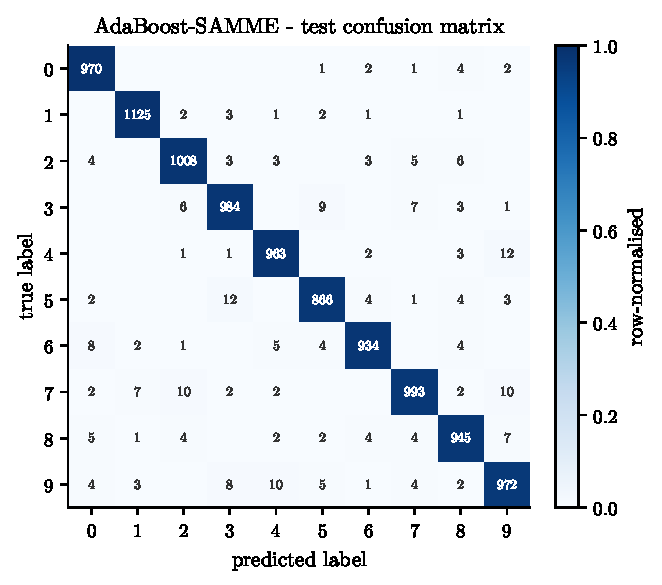
\includegraphics[width=\linewidth]{../results/figures/confusion_adaboost.pdf}\caption{AdaBoost}\end{subfigure}\hspace{0.03\textwidth}
\begin{subfigure}{0.325\textwidth}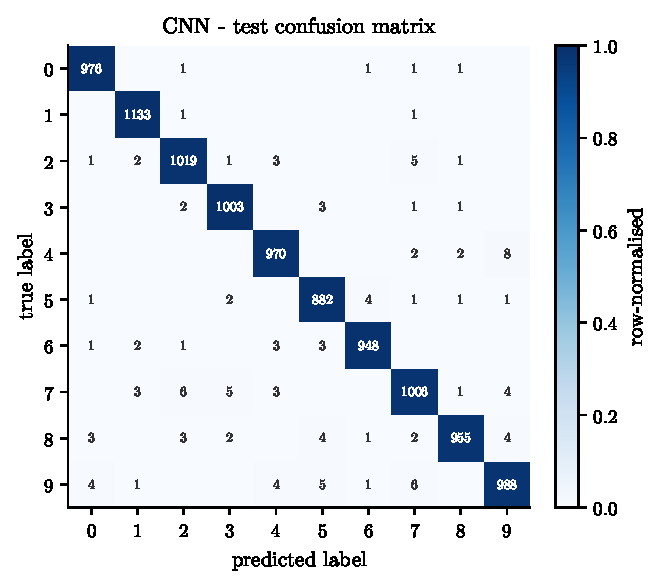
\includegraphics[width=\linewidth]{../results/figures/confusion_cnn.pdf}\caption{CNN}\end{subfigure}
\caption{Ma trận nhầm lẫn trên tập test (hàng: chữ số thật; cột: dự đoán). Ma trận của train và validation nằm trong \texttt{results/final/*.json}.}
\label{fig:confusion}
\end{figure}

Cả năm mô hình đều nhầm nhiều nhất ở những cặp có nét chung (\cref{fig:confusion}): $4\to9$ là cặp lớn nhất của Naïve Bayes (284 trong \errorsNB{} lỗi), softmax, AdaBoost và CNN; MLP nhầm nhiều nhất $7\to9$. Các cặp $5\to3$ và $7\to9$ cũng nằm trong ba cặp đầu của nhiều mô hình.

\subsection{Ảnh hưởng của siêu tham số}
\begin{figure}[tbp]
\centering
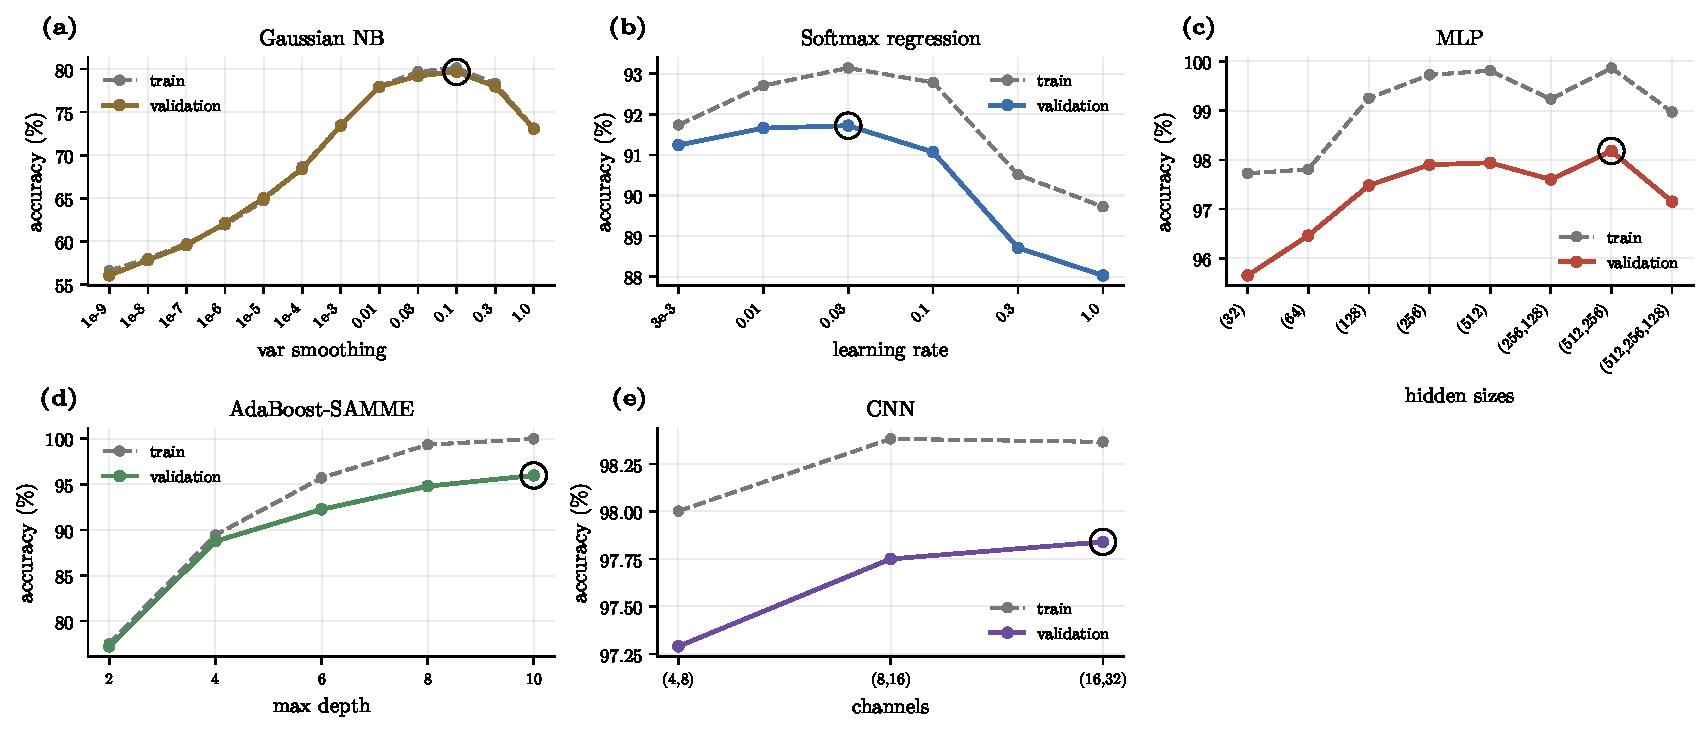
\includegraphics[width=\textwidth]{../results/figures/key_sweeps.pdf}
\caption{Accuracy train và validation theo siêu tham số quan trọng nhất của từng mô hình; vòng tròn đánh dấu giá trị được chọn. Các lượt quét chạy tuần tự nên phần còn lại của cấu hình ở giá trị tốt nhất tìm được trước đó.}
\label{fig:sweeps}
\end{figure}

\Cref{fig:sweeps} cho thấy: (a) Naïve Bayes: \texttt{var\_smoothing} tăng từ $10^{-9}$ lên $0.1$ làm validation tăng từ $56.05\%$ lên $79.67\%$, train và validation gần trùng nhau nên mô hình bị giới hạn bởi giả thiết độc lập chứ không do overfitting; (b) softmax: tốc độ học $0.03$ tốt nhất, giá trị lớn hơn làm cả train lẫn validation giảm; (c) MLP: hai lớp ẩn $(512,256)$ đạt $98.18\%$, hơn một lớp ẩn $(97.94\%)$ và ba lớp ẩn $(97.15\%)$; (d) AdaBoost: validation tăng đơn điệu theo độ sâu cây; (e) CNN: $(16,32)$ kênh cho validation cao nhất. Với AdaBoost (độ sâu 10) và CNN, giá trị tốt nhất nằm ở mép khoảng đã quét nên có thể chưa tối ưu. Số epoch của MLP do dừng sớm quyết định (dừng ở epoch 14, khôi phục epoch 9), số vòng boosting là 393.

\subsection{Thời gian huấn luyện, thời gian dự đoán và đối chiếu scikit-learn}
\begin{table}[tbp]
\centering\small
\begin{tabular}{lrrrr}
\toprule
Mô hình & Huấn luyện (s) & Dự đoán $10\,000$ ảnh (s) & Một ảnh (ms) & Tệp xuất (KiB) \\
\midrule
Gaussian NB & 0.4 & 0.226 & 0.076 & 62 \\
Softmax regression & 12.7 & 0.024 & 0.010 & 31 \\
MLP & 11.0 & 0.051 & 0.042 & 2\,094 \\
AdaBoost-SAMME & 817.9 & 0.751 & 18.705 & 9\,457 \\
CNN & 143.0 & 1.163 & 0.315 & 223 \\
\bottomrule
\end{tabular}

\caption{Chi phí trên CPU: huấn luyện trên $50\,000$ ảnh, dự đoán $10\,000$ ảnh test, thời gian một ảnh và kích thước tệp mô hình xuất ra.}
\label{tab:cost}
\end{table}

AdaBoost đắt nhất (\cref{tab:cost}): \fitADA\,s huấn luyện và \latADA\,ms cho một ảnh, vì phải duyệt $393$ cây (một phần do vòng lặp Python trong cài đặt). Naïve Bayes và softmax rẻ nhất. CNN chậm hơn MLP khoảng $13$ lần khi huấn luyện và $7$ lần khi dự đoán.

\begin{table}[tbp]
\centering\small
\begin{tabular}{lrrrrr}
\toprule
Mô hình & Test (ours) & Test (sklearn) & $|\Delta|$ & Fit ours (s) & Fit sklearn (s) \\
\midrule
Gaussian NB & 81.32 & 81.32 & 0.00 & 0.4 & 0.2 \\
Softmax regression & 92.52 & 91.86 & 0.66 & 12.7 & 154.6 \\
MLP & 98.24 & 98.02 & 0.22 & 11.0 & 57.8 \\
AdaBoost-SAMME & 97.60 & 97.50 & 0.10 & 817.9 & 1892.8 \\
\bottomrule
\end{tabular}

\caption{Bản tự cài đặt và scikit-learn với cùng siêu tham số: accuracy test (\%), hiệu tuyệt đối và thời gian huấn luyện.}
\label{tab:sklearn}
\end{table}

Naïve Bayes trùng khớp với scikit-learn (\cref{tab:sklearn}). Ba mô hình còn lại lệch từ $0.10$ đến $0.66$ điểm: softmax của nhóm cao hơn vì scikit-learn (L-BFGS) chạm giới hạn vòng lặp mà chưa hội tụ, còn nhóm dừng ở epoch chọn bằng validation; MLP chênh $0.22$ điểm; AdaBoost chênh $0.10$ điểm, hai bản dùng cách chia nút khác nhau (histogram so với ngưỡng chính xác) nên thời gian không so sánh trực tiếp được.

\subsection{So sánh ưu và nhược điểm}
\begin{table}[H]
\centering\footnotesize
\renewcommand{\arraystretch}{1.1}
\newcolumntype{L}[1]{>{\raggedright\arraybackslash}p{#1}}
\begin{tabular}{@{}L{2.0cm}L{3.9cm}L{3.9cm}L{4.5cm}@{}}
\toprule
Mô hình & Độ chính xác & Thời gian huấn luyện và dự đoán & Khả năng giải thích \\
\midrule
Naïve Bayes & Thấp nhất (\accTestNB\%): giả thiết độc lập bị mâu thuẫn bởi tương quan giữa các pixel kề nhau. & Rẻ: \fitNB\,s huấn luyện, \latNB\,ms mỗi ảnh. & Tham số $\mu_{kj},\sigma_{kj}$ là ảnh trung bình và phương sai theo lớp, đọc trực tiếp. \\
Softmax & \accTestSM\%; train chỉ $93.62\%$, bị giới hạn bởi biên tuyến tính. & Dự đoán nhanh (\latSM\,ms mỗi ảnh); huấn luyện \fitSM\,s. & Trọng số theo lớp vẽ được thành ảnh; $x_iW_{ik}$ phân rã chính xác điểm số. \\
MLP & \accTestMLP\%; chênh train--test $1.63$ điểm. & \fitMLP\,s huấn luyện, \latMLP\,ms mỗi ảnh. & Khó: đơn vị ẩn gần như không đọc được bằng mắt. \\
AdaBoost-SAMME & \accTestADA\%, gần MLP; train $100\%$. & Đắt nhất: \fitADA\,s huấn luyện, \latADA\,ms mỗi ảnh. & Bản đồ tần suất pixel được cây dùng; điểm là tỉ lệ phiếu, chưa phải xác suất. \\
\bottomrule
\end{tabular}
\caption{Ưu và nhược điểm của bốn mô hình theo bốn tiêu chí của đề bài (số liệu từ \cref{tab:accuracy,tab:cost}; nhận xét về khả năng giải thích là định tính, \cref{fig:interp}).}
\label{tab:summary}
\end{table}

\begin{figure}[H]
\centering
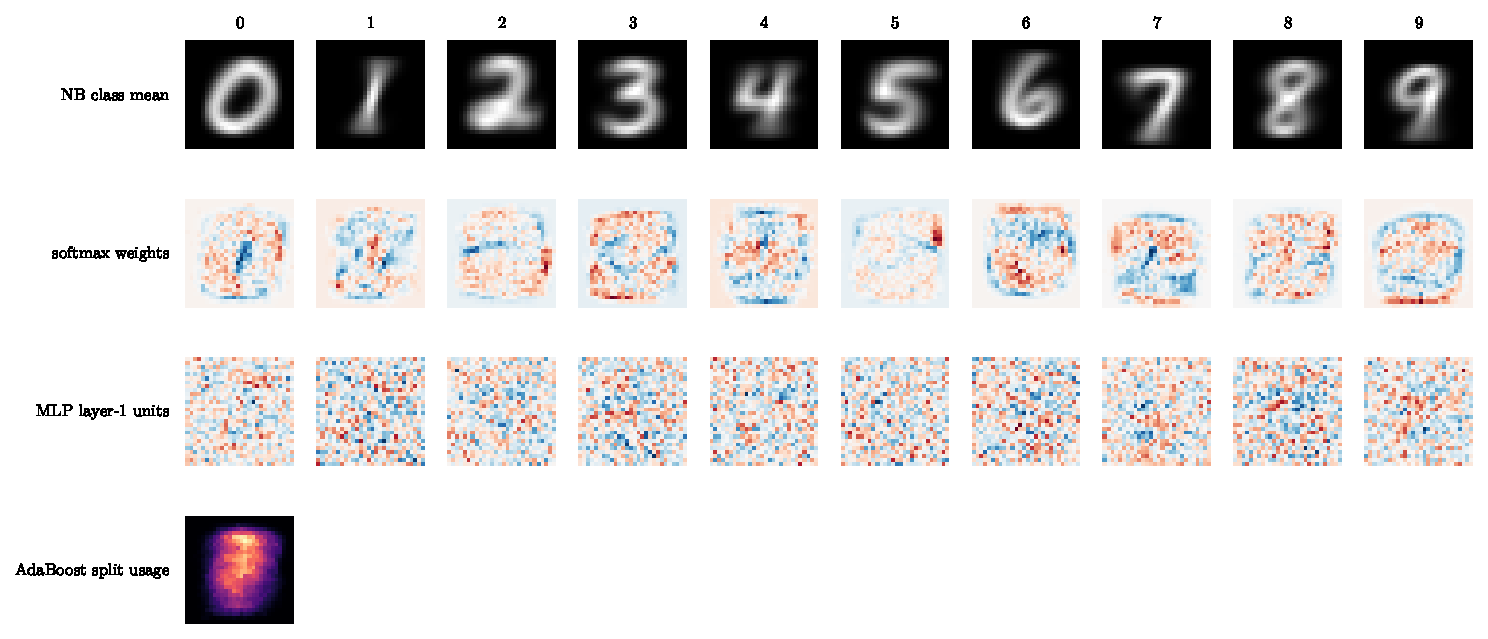
\includegraphics[width=0.78\textwidth]{../results/figures/interpretability.pdf}
\caption{Tham số hoặc thống kê của từng mô hình: ảnh trung bình theo lớp (Naïve Bayes), trọng số theo lớp (softmax; đỏ dương, xanh âm), các đơn vị ẩn đầu tiên của MLP và tần suất pixel được dùng để chia nhánh (AdaBoost).}
\label{fig:interp}
\end{figure}
